

Bureaucracy is a consistent and pervasive challenge in modern society. You have direct experience with bureaucracy and are familiar with complaints about bureaucracy. You probably don't consider yourself a bureaucrat.

This book is intended to alter your view of bureaucracy. This book starts with an unconventional definition and then uses the definition to explain the necessity of various aspects of bureaucracy. Having identified specific challenges, the book serves as a guide for how you can be effective. 

A guide for situations you haven't been in before can decrease your anxiety by making the unfamiliar less intimidating. 
A guide labels patterns and provides context for your observations. 
Recognizing a familiar challenge can be preferable to the uncertainty of facing a novel scenario. An unfamiliar situation means not knowing how to start and not knowing the potential paths to success. In contrast, a challenge you understand can feel less burdensome. 
% 2023-01-05: Alicia@Upwork added the following sentence
Even if you have not faced the particular challenge before, a guide can make that new challenge seem familiar and manageable. 
Having a guide doesn't make your life easy -- even a challenge that is understood requires creativity and effort.

%If you don't think of yourself as a bureaucrat, I hope to change your mind on this essential topic. 

Having a guide isn't helpful if you find the topic repulsive.
Negative impressions of bureaucracy are common. The word
%bureaucracy 
% 2022-07-09: Jonah@upwork advocates removing this use
evokes reactions of disgust, primarily driven by how individuals have experienced bureaucracy.
The results of bureaucracy can appear idiotic -- 
% 2023-01-05: Alicia@Upwork says be more specific
wasting time and resources or causing harm to people.
%\footnote{In some dialects of Romani language, the word bureaucracy translates as ``the violence of paper.''}
%TODO: citation needed for Romani translation claim
% https://github.com/processempathy/bureaucracy-guidebook/issues/24
Bureaucracy is even regarded as dangerous to society.\footnote{``The only thing that saves us from the bureaucracy is inefficiency. An efficient bureaucracy is the greatest threat to liberty." (Eugene McCarthy, 1979~\cite{1979_McCarthy})}
% Time magazine, Feb. 1979
% https://en.wikiquote.org/wiki/Eugene_McCarthy
% https://time.com/vault/issue/1979-02-12/page/83/
I have bad news for you if you have a negative impression of bureaucracy: bureaucracy is vital to society. 

Having a precise definition of bureaucracy enables a more nuanced discussion.\nolinebreak 
\begin{quote}
\textbf{Definition}: 
\iftoggle{glossarysubstitutionworks}{\Gls{bureaucracy}}{Bureaucracy}
is the process of enacting policies through subjective decisions made by a person, typically in the context of managing access to a shared resource. Three roles are present: policy maker, bureaucrat, and subject.
\end{quote}

% Effective bureaucracy is  to modern society.
%Organizations have an insatiable need for members to perform a variety of tasks.

The concepts and techniques in this book are derived from this definition. For example, in an organization comprised of bureaucrats no one member knows everything and no one person decides everything, so bureaucracy relies on distributed knowledge and distributed decision-making amongst people with distinct roles.
%The resources managed by an organization can be either tangible or intangible. 
For more exploration of this definition, see the section ``\hyperref[sec:define-bureaucracy]{What is Bureaucracy?}''%
\iftoggle{haspagenumbers}{ on page~\pageref{sec:define-bureaucracy}.}{}


You can learn to skillfully navigate bureaucracy by using the techniques in this book. A skilled bureaucrat is more effective. That improvement enhances the organization you are a member of. Modern society is an interwoven fabric of organizations, with  bureaucracy being the crucial material.
Rather than ponder societal-scale concerns, this book focuses on the complicated and typical experience of a bureaucrat. 

The framing of how you think about bureaucracy shapes what action you feel is relevant for changing your environment. 
Suppose your assumptions are wrong about how the system of bureaucracy works. Then you will be trying to change the system to meet your incorrect expectations and your actions are likely to be wasted effort tackling irrelevant aspects. 
An accurate understanding of bureaucracy allows you to be more effective and your changes to the system are more likely to succeed. 


As an example of how the above definition is distinct from conventional definitions,%
\footnote{\href{https://www.merriam-webster.com/dictionary/bureaucracy}{Merriam-Webster's definition} focuses on government; the \href{https://en.wikipedia.org/wiki/Bureaucracy}{Wikipedia entry}
\index{Wikipedia!bureaucracy@\string\href{https://en.wikipedia.org/wiki/Bureaucracy}{bureaucracy}}
acknowledges non-governmental bureaucracy.} I view government as an instance of where bureaucracy occurs -- rather than equating government to bureaucracy. By the definition in this book bureaucracy is not limited to governments. I use ``organization'' to encompass governments, corporations, non-profits, or any collection of people working together. As a consequence, many people are bureaucrats. 


The widely-held negative connotation of bureaucracy may lead you to reject the label of bureaucrat. Your recognition of your status as a bureaucrat matters even if you intentionally reject the label or do not recognize that you are a bureaucrat. How you behave and what you think your responsibilities are depend on how you label yourself.
% If you do not recognize that you are bureaucrat, you're less likely to be successful interacting with those around you. 
If you don't think of yourself as a bureaucrat, then you won't be able to distinguish what is your fault, what is the fault of your coworkers, what is the fault of management, and what is intrinsic to bureaucracy. 

Reasoning about bureaucracy is an accessible topic for every reader because we each have personal experiences.
A commonly held view is that the bureaucracies we work within are broken: participants are harmed and there is inequality. 
A counterargument is that the bureaucratic behavior observed is how the system was designed to work. There is a third argument: bureaucratic systems work in a degraded mode -- they are less efficient than what is possible. 
In this book I set aside the macro-scale questions of bureaucracy like the three arguments above and focus on the human-scale interactions that give rise to bureaucracy. Rather than complain about systemic problems, this book provides you with practical actions for situations you encounter.

Even people who are smart (e.g., they know history, they have memorized state capitals, they can do math) can struggle when faced with complex, large-scale distributed systems comprised of humans. Thinking about complex, large-scale systems is not part of the conventional education curriculum. This book will help you learn about bureaucracy, increase your ability to identify patterns, and apply relevant techniques. The pervasiveness of bureaucracy means the opportunities to apply the skills you learn in this book are many -- at your job, at the grocery store, in negotiations with your family.


The difficulties of bureaucracy are central to large societies that have complicated dependencies on the interactions of many people. From foundational services like the delivery of water and removal of sewage, to advanced manufacturing that relies on long supply chains, bureaucracy is essential.  The challenge of bureaucracy affects governments and companies in different societies of all scales. And bureaucracy is durable -- it has existed for thousands of years. Because bureaucracy is pervasive, tackling the topic of bureaucracy is exciting and crucial. The excitement comes from the opportunities available for the many potential improvements.
%I enjoy pondering hard problems and then leveraging insights gained from reflection.
Being an effective bureaucrat is important because bureaucracy can be a \href{https://en.wikipedia.org/wiki/Force_multiplication}{force multiplier}\iftoggle{WPinmargin}{\marginpar{$>$Wikipedia: Force multiplication}}{}
\index{Wikipedia!force multiplication@\href{https://en.wikipedia.org/wiki/Force_multiplication}{force multiplication}}
beyond what one person could achieve on their own.

% there's no avoiding the issue
Everyone is a bureaucrat because there are few alternatives to bureaucracy for a society constrained by finite resources. Gaining skills in navigating bureaucracy is helpful both for your happiness and the improved functioning of society. That may seem abstract and lofty, but the situation is inescapable: you are a member of society and benefit from participating in society. 


% Who this book is for

% from https://graphthinking.blogspot.com/2021/07/bureaucracy-book-outline.html
This book is for you if you are curious about the complex world we live in,  if you are thinking about how to contribute to society,  if you want your employment to have impact, or if your job is different from what you expected. This book will help you understand why and how innovation is suffocated within bureaucratic organizations. Understanding the challenges means you can design ideas that are more likely to succeed.


% What you should expect reading this book: 
Every person in society is a participant in bureaucracy. The purpose of this book is to decrease the surprise of that experience and better prepare you emotionally and intellectually for the toil of being a bureaucrat. You can improve your skills as a bureaucrat with focused reflection and a good guide like this book. 

The topic of bureaucracy spans academic disciplines - \href{https://en.wikipedia.org/wiki/Psychology}{psychology},
\index{Wikipedia!psychology@\href{https://en.wikipedia.org/wiki/Psychology}{psychology}}\iftoggle{WPinmargin}{\marginpar{$>$Wikipedia: psychology}}{}
\href{https://en.wikipedia.org/wiki/Sociology}{sociology},
\index{Wikipedia!sociology@\href{https://en.wikipedia.org/wiki/Sociology}{sociology}}
\href{https://en.wikipedia.org/wiki/Organizational_behavior}{organizational dynamics},
\index{Wikipedia!organizational behavior@\href{https://en.wikipedia.org/wiki/Organizational_behavior}{organizational behavior}}
\href{https://en.wikipedia.org/wiki/Public_administration}{public administration}, 
\index{Wikipedia!public administration@\href{https://en.wikipedia.org/wiki/Public_administration}{public administration}}
\href{https://en.wikipedia.org/wiki/Anthropology}{anthropology},
\index{Wikipedia!anthropology@\href{https://en.wikipedia.org/wiki/Anthropology}{anthropology}}
and  
\href{https://en.wikipedia.org/wiki/Political_science}{political science}. 
\index{Wikipedia!political science@\href{https://en.wikipedia.org/wiki/Political_science}{political science}}
Most bureaucrats have no formal training in any of these domains. This book is not written from an academic perspective; it is written by a practicing bureaucrat to serve as a guide to be read by bureaucrats. 


% What is the benefit of reading this book?
As a result of reading this book, you will be better able to recognize and navigate complex human interactions within your career and outside of work. Perspectives offered in this book can benefit you directly, whether by promotion in rank or title, increase in pay, successful completion of a project, or through decreased stress derived from an improved understanding of  bureaucracy. Being a more effective bureaucrat can also positively effect the causes you care about and the people you engage with.



\subsection*{What this Book is Not}

This book is not a defense of bureaucracy, nor is it intended to disparage bureaucrats or the system of bureaucracy. Instead, this book is a guide to bureaucracy-as-it-is. There are no hacks presented for circumventing bureaucracy. Instead, this book provides advice on being an effective member of a bureaucratic organization.

This book does not focus on leadership, managing a team, being a team member, planning, time management, project management, advancing your career, promotions, or self-improvement. In the process of being a better bureaucrat, some lessons may apply in those domains.


Nothing in this book is domain-specific, nothing is tied to the engineering of products, and nothing applies solely to science research or policy development. However, skills associated with being an effective bureaucrat do translate into other domains.


This book does not discuss work conditions, pay, benefits, or retirement plans. If you are seeking a competitive advantage that might result in improved outcomes, learning to navigate bureaucracy helps.


This book doesn't focus on citizens, political 
\iftoggle{glossarysubstitutionworks}{\glspl{policymaker}}{policymakers}, oversight (e.g., Congress at the state or federal level, Inspectors General), 
competing organizations, contracts, the budget of an organization, fines and other regulatory punishments resulting from bureaucracy, policy enforcement, specific policies and regulations, formal arbitration or judicial resolution of disputes. For observations on those topics, see Wilson's \textit{Bureaucracy}~\cite{1991_Wilson}. 


This book doesn't discuss discrimination or harassment. I neglect differences in experience based on race, gender, or socioeconomic status. This book doesn't discuss bad coworkers, abusive bosses, psychological defects of individuals, or malicious intent. I assume no traitors, spies, \iftoggle{WPinmargin}{\marginpar{$>$Wikipedia: saboteurs}}{}
or saboteurs~\cite{1944_War_Dept}. I do not discuss \href{https://en.wikipedia.org/wiki/Dark_pattern}{dark patterns}; 
\index{Wikipedia!dark pattern@\href{https://en.wikipedia.org/wiki/Dark_pattern}{dark pattern}}
issues like lying, bribery~\cite{2021_Ang}, and criminal behavior are not discussed. Those aspects happen whenever people interact, so  the challenges of intentional defectors are not specific to bureaucracy. 

Bureaucracy is not a manifestation of incompetence, laziness, or mistakes.
% removed "malicious actors" from list
% malice
Even with well-trained bureaucrats trying to help other people, challenges arise when people interact to manage access to a shared resource. 
%The Good Samaritan is more applicable than a rational actor model
Sources of friction in a well-run bureaucracy stem from  ambiguity, conflicting incentives, finite attention, and inadequate resources. Bureaucracy is only necessary because shared resources are scarce. There's not enough to satisfy the needs of the community, leading to contention. Therefore distributed decision-making and distributed knowledge are relevant for the allocation of those resources.


Focusing on the morals of organizations or bureaucrats~\cite{2009_Jackall} is less compelling than studying bureaucracy because norms (i.e., expectations for individuals and organizations) shift over time, while bureaucracy is persistent. 
In this book I focus on culturally invariant aspects of bureaucracy. 


\subsection*{Assumptions}
As a way of limiting the complexity of this book, I assume you are honest and that other people are honest. 
%That isn't always applicable, but I'm aiming to describe __(?)
I assume bureaucrats strive for fairness, though the definition of fairness may vary from bureaucrat to bureaucrat. 
The complexities of bureaucracy arise even with these simplifying assumptions.% and unaddressed topics. 
My guidance on how to be an effective bureaucrat applies to  bureaucracy that was intended to be helpful (rather than malicious).



% Source of this content: 
This book is based on personal experience operating in multiple large organizations and small teams, reading published books and papers, and insight from fellow bureaucrats. Informal surveys were conducted but are not foundational for claims made in this book.%
\iftoggle{WPinmargin}{\marginpar{$>$Wikipedia: blinded-experiment}}{}
No \href{https://en.wikipedia.org/wiki/Blinded_experiment}{double-blind}%
\index{Wikipedia!blinded experiment@\href{https://en.wikipedia.org/wiki/Blinded_experiment}{blinded experiment}}
experiments were conducted. 
% my experience
% I wrote this book for a younger version of me.
% When I first started my job in a large organization I recognized differences between the expectations of the education system I had left and the challenges of a professional environment. 
I have tried to learn from my mistakes by reflecting on my (in)actions and the consequences. This haphazard approach has been an expensive education. My mistakes delayed progress and damaged relationships. This book  provides generalizations from my experiences that might benefit the reader. My hope for this guide is to decrease your surprise when you encounter what would have been novel situations.

\ \\

% How the book should be read: 
Reading this book front-to-back is the default option, but not required. The dependencies of topics are not sequential -- see Figure~\ref{fig:core-concepts}.

\begin{figure}[ht]
    \centering
    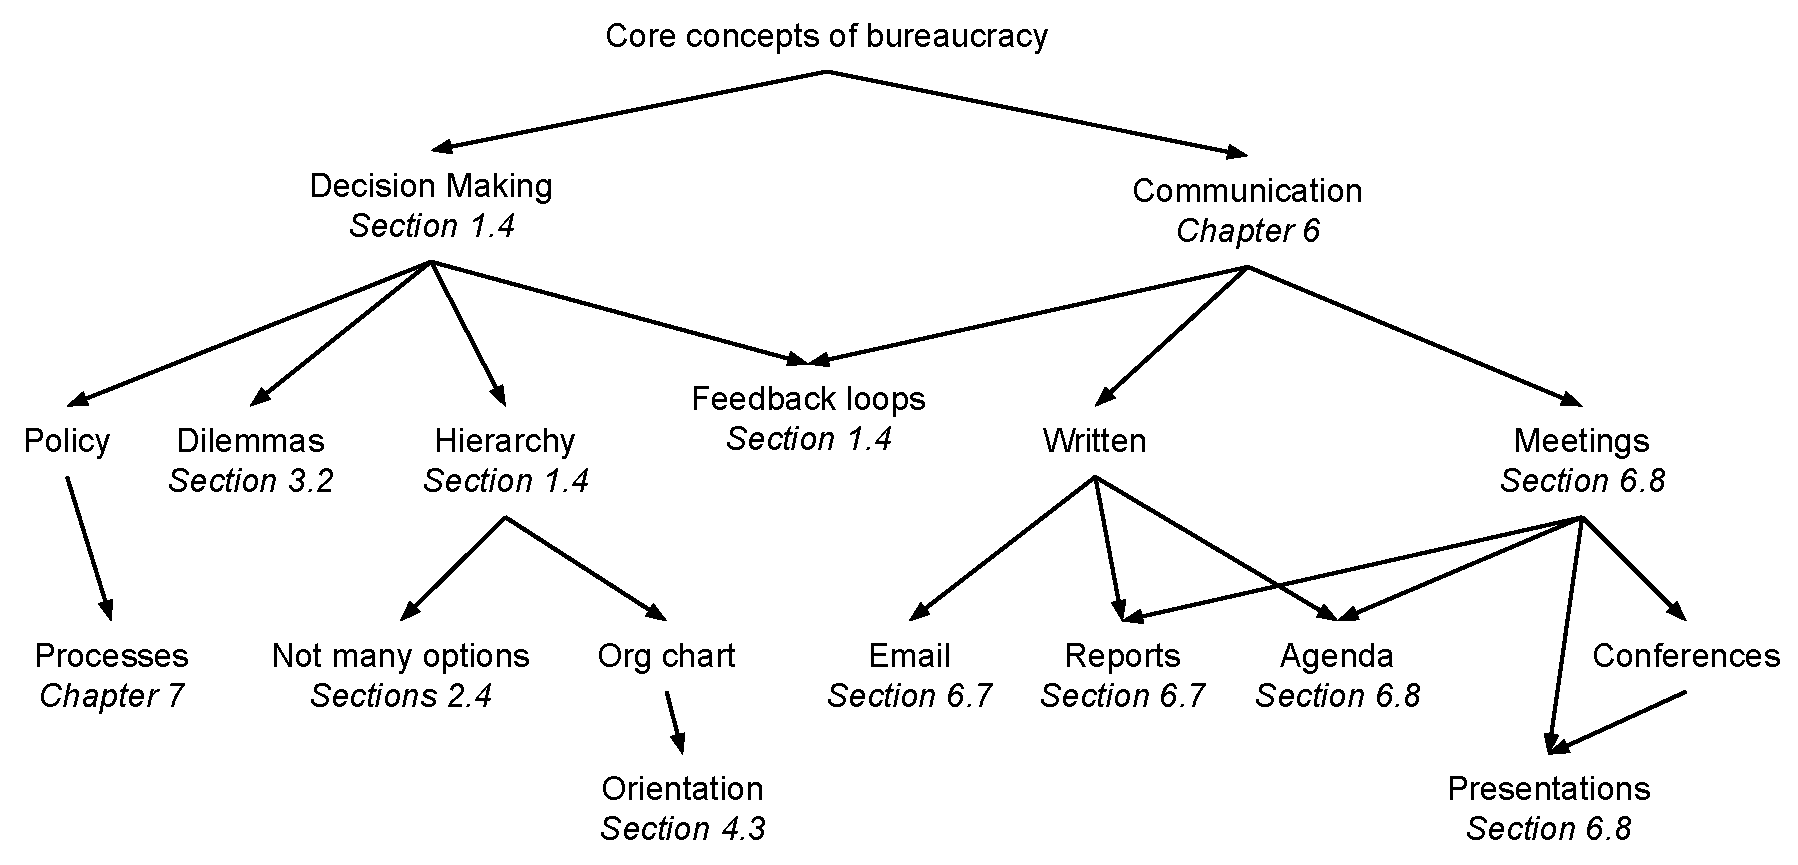
\includegraphics[width=1\textwidth]{images/core_concepts_map.pdf}
    \caption{Relation of the concepts related to bureaucracy discussed in this book.}
    % TODO (aspirational): generate diagram from Latex
    \label{fig:core-concepts}
\end{figure}

% 2022-03-27: BHP was not impressed by the options on https://texample.net//tikz/examples/tag/graphs/ including the "mindmap" option
% this looks better: http://randomresearchdata.blogspot.com/2013/12/tikz-simple-decision-tree-or-cart-tree.html
% see https://texample.net/tikz/examples/feature/trees/

%\begin{tikzpicture}[main/.style = {draw, circle}] 
%\node[main] (1) {Core Concepts}; 
%\node[main] (2) [above right of=1] {Decision-making}; 
%\draw[->] (1) -- (2);
%\end{tikzpicture} 

The approach in this book is to view bureaucracy from a few perspectives. The first is a conceptual view focused on the \hyperref[sec:define-bureaucracy]{definition of bureaucracy} %\iftoggle{haspagenumbers}{ (page~\pageref{sec:define-bureaucracy})}{}
in terms of managing shared resources. The second view is structural (e.g., hierarchy, meetings). The \hyperref[sec:fundamentals-of-b]{essentials of bureaucracy}%
\iftoggle{haspagenumbers}{ (page~\pageref{sec:fundamentals-of-b})}{} 
will be familiar to experienced bureaucrats. 
The third view is based on the experience of a practicing bureaucrat -- 
\hyperref[sec:dilemma-trilemma]{dilemmas}\iftoggle{haspagenumbers}{~(page~\pageref{sec:dilemma-trilemma}),}{,}
\hyperref[sec:unavoidable-hazards]{unavoidable hazards}\iftoggle{haspagenumbers}{~(page~\pageref{sec:unavoidable-hazards}),}{,}
and 
\hyperref[sec:effective-bureaucrat]{tips on how to be effective}\iftoggle{haspagenumbers}{~(page~\pageref{sec:effective-bureaucrat}).}{.}

%The three productive views of bureaucracy (concept, structure, experience) are contrasted with~\hyperref[sec:alternative-views-from-within]{how other bureaucrats view bureaucracy} and~\hyperref[sec:models-of-bureaucracy]{other models of bureaucracy}.

Chapters~\ref{sec:introduction} %\iftoggle{haspagenumbers}{(page~\pageref{sec:introduction}) }{}
through~\ref{sec:why-bur-hard} %\iftoggle{haspagenumbers}{(page~\pageref{sec:why-bur-hard}) }{}
provide background context for bureaucracy. 
Chapters~\ref{sec:individual-in-org} %\iftoggle{haspagenumbers}{(page~\pageref{sec:individual-in-org}) }{}
through~\ref{sec:process} %\iftoggle{haspagenumbers}{(page~\pageref{sec:process}) }{}
are the guide. 
You can read each chapter of the guide independently. 

The freely available electronic versions of this book (including 
\index{Wikipedia!PDF@\href{https://en.wikipedia.org/wiki/PDF}{PDF}}\iftoggle{WPinmargin}{\marginpar{$>$Wikipedia: PDF}}{}
\href{https://en.wikipedia.org/wiki/PDF}{PDF}, 
\index{Wikipedia!HTML@\href{https://en.wikipedia.org/wiki/HTML}{HTML}}
\href{https://en.wikipedia.org/wiki/HTML}{HTML}, and 
\index{Wikipedia!EPUB@\href{https://en.wikipedia.org/wiki/EPUB}{EPUB}}
\href{https://en.wikipedia.org/wiki/EPUB}{EPUB} 
formats) have hyperlinks in the text. Light-blue hyperlinks reference external resources like Wikipedia, while dark-blue links reference material within the guide such as the glossary. 
%The PDF and printed versions have notes in the margin to help identify the links.


\ \\

% as per https://tex.stackexchange.com/q/393238/235813
\begin{flushright}
Ben Payne\\
\today\\
United States of America\\
Earth
\end{flushright}


